\documentclass[border=10pt]{standalone}
\usepackage{amsmath,amssymb}
\usepackage{xcolor}
\usepackage{tikz}
\usetikzlibrary{arrows.meta,calc,decorations.pathreplacing,decorations.pathmorphing,patterns,shapes.geometric,positioning,shadings}

\definecolor{photonred}{HTML}{C0392B}
\definecolor{cathodegray}{HTML}{333333}
\definecolor{linenavy}{HTML}{1F3A68}
\definecolor{auxgray}{HTML}{888888}

\begin{document}
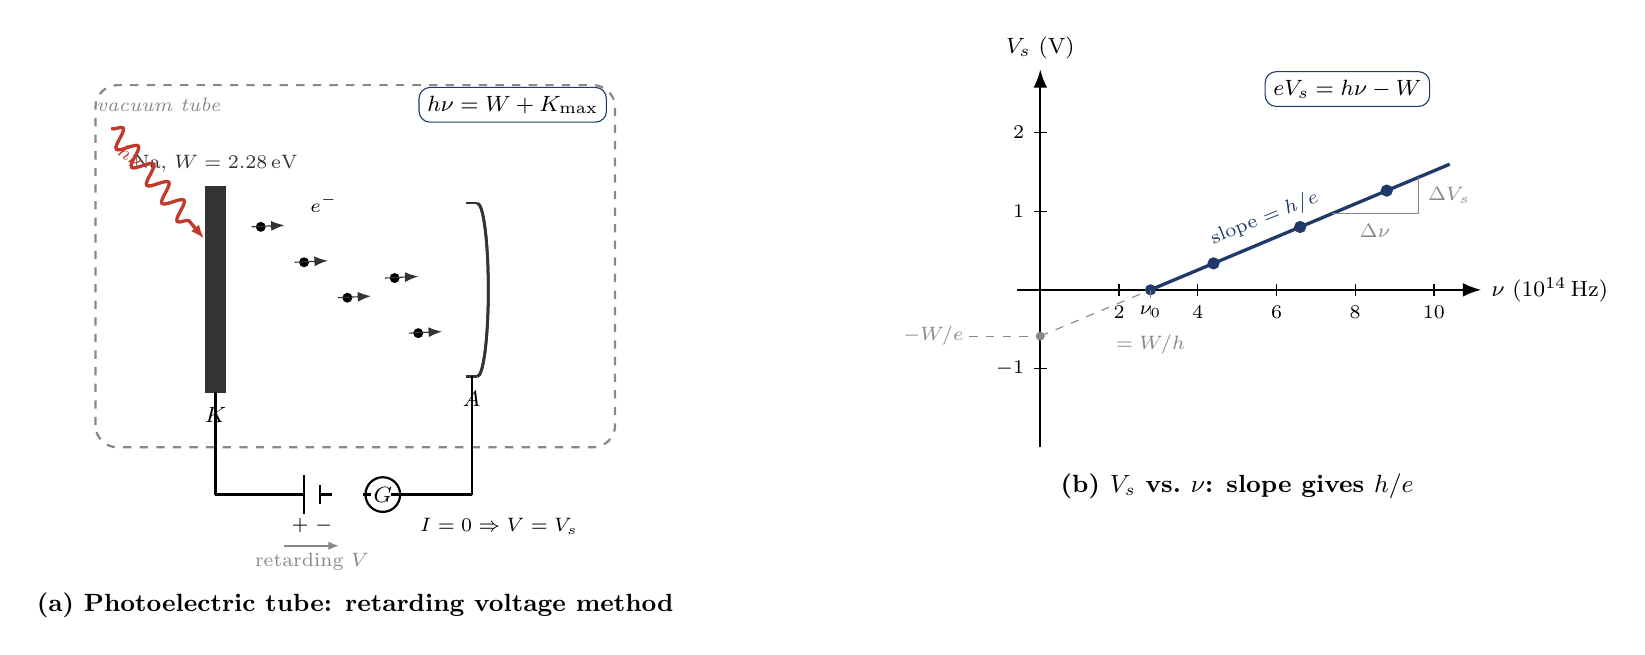
\begin{tikzpicture}[>=Latex, font=\small]

% ============================================================
% LEFT: Photoelectric tube circuit schematic
% ============================================================
\begin{scope}[shift={(0,0)}]

% Vacuum tube outline (dashed rounded rectangle)
\draw[dashed, rounded corners=8pt, auxgray, thick]
  (-3.2,-2.0) rectangle (3.4,2.6);
\node[auxgray, font=\scriptsize\itshape] at (-2.4,2.35) {vacuum tube};

% Cathode K (dark grey vertical bar)
\fill[cathodegray] (-1.8,-1.3) rectangle (-1.55,1.3);
\draw[cathodegray, thick] (-1.8,-1.3) rectangle (-1.55,1.3);
\node[below=2pt, font=\footnotesize] at (-1.675,-1.3) {$K$};
\node[above=2pt, font=\scriptsize, text=cathodegray]
  at (-1.675,1.3) {Na, $W=2.28\,\mathrm{eV}$};

% Incident photon: red wavy arrow from upper-left to cathode
\draw[photonred, line width=1.2pt, decorate,
      decoration={snake, amplitude=1.2mm, segment length=3mm,
                  post length=2.5mm},
      -{Latex[length=5pt]}]
  (-3.0,2.05) -- (-1.82,0.65);
\node[photonred, font=\scriptsize, rotate=-35]
  at (-2.75,1.7) {$h\nu$};

% Electrons flying rightward from cathode toward anode
\foreach \y/\x in {0.8/-1.1, 0.35/-0.55, -0.1/0.0, 0.15/0.6, -0.55/0.9}{
  \fill[black] (\x,\y) circle (1.8pt);
  \draw[->, thin, black!80]
    (\x-0.12,\y) -- (\x+0.3,\y+0.02);
}
\node[black, font=\scriptsize] at (-0.3,1.1) {$e^{-}$};

% Anode A (ring, drawn as two short vertical arcs bridged top/bottom)
\draw[cathodegray, line width=1pt] (1.65,-1.1) arc (-90:90:0.14 and 1.1);
\draw[cathodegray, line width=1pt] (1.65,-1.1) arc (270:90:-0.14 and 1.1);
\draw[cathodegray, thick] (1.51,-1.1) -- (1.65,-1.1);
\draw[cathodegray, thick] (1.51,1.1) -- (1.65,1.1);
\node[below=2pt, font=\footnotesize] at (1.58,-1.1) {$A$};

% Wires leaving the tube downward
\draw[thick] (-1.675,-1.3) -- (-1.675,-2.6);
\draw[thick] (1.58,-1.1) -- (1.58,-2.6);

% Horizontal wires to battery and galvanometer
\draw[thick] (-1.675,-2.6) -- (-0.7,-2.6);
\draw[thick] (0.55,-2.6) -- (1.58,-2.6);

% Battery (reverse voltage V) between (-0.7,-2.6) and (-0.2,-2.6)
\draw[thick] (-0.55,-2.85) -- (-0.55,-2.35);   % long plate (+)
\draw[thick] (-0.35,-2.72) -- (-0.35,-2.48);   % short plate (-)
\draw[thick] (-0.7,-2.6) -- (-0.55,-2.6);
\draw[thick] (-0.35,-2.6) -- (-0.2,-2.6);
\node[font=\scriptsize] at (-0.6,-3.0) {$+$};
\node[font=\scriptsize] at (-0.3,-3.0) {$-$};
% Reverse voltage arrow and label
\draw[-{Latex[length=4pt]}, auxgray, thick]
  (-0.8,-3.25) -- (-0.1,-3.25);
\node[auxgray, font=\scriptsize] at (-0.45,-3.45) {retarding $V$};

% Ammeter/Galvanometer G
\draw[thick] (0.2,-2.6) -- (0.3,-2.6);
\draw[thick] (0.45,-2.6) circle (0.22);
\node[font=\footnotesize] at (0.45,-2.6) {$G$};
\draw[thick] (0.67,-2.6) -- (0.7,-2.6);
\node[font=\scriptsize, anchor=west]
  at (0.8,-3.0) {$I=0 \Rightarrow V=V_{s}$};

% Corner formula: Einstein equation
\node[draw=linenavy, rounded corners, line width=0.4pt,
      fill=white, font=\footnotesize, inner sep=3pt]
  at (2.1,2.35) {$h\nu = W + K_{\max}$};

% Panel label
\node[font=\small\bfseries] at (0.1,-4.0)
  {(a) Photoelectric tube: retarding voltage method};

\end{scope}

% ============================================================
% RIGHT: V_s vs nu linear plot
% ============================================================
\begin{scope}[shift={(8.8,0)}]

% Axes
\draw[->, thick] (-0.3,0) -- (5.6,0)
  node[right, font=\footnotesize] {$\nu\ (10^{14}\,\mathrm{Hz})$};
\draw[->, thick] (0,-2.0) -- (0,2.8)
  node[above, font=\footnotesize] {$V_{s}\ (\mathrm{V})$};

% x-axis ticks (each unit = 2e14 Hz)
\foreach \x/\lab in {1/2, 2/4, 3/6, 4/8, 5/10}{
  \draw (\x,0.08) -- (\x,-0.08);
  \node[below, font=\scriptsize] at (\x,-0.08) {\lab};
}
% y-axis ticks
\foreach \y in {1, 2}{
  \draw (0.08,\y) -- (-0.08,\y);
  \node[left, font=\scriptsize] at (-0.08,\y) {\y};
}
\draw (0.08,-1) -- (-0.08,-1);
\node[left, font=\scriptsize] at (-0.08,-1) {$-1$};

% Line parameters (schematic; not numerically exact):
% Choose nu_0 = 1.4 (on x-axis, i.e. 2.8e14 Hz threshold), slope = 0.42 V/(x-unit)
% y-intercept = -slope*nu_0 = -0.588 V -> shown as -W/e
\def\nuz{1.4}
\def\slope{0.42}

% Dashed extrapolation from y-intercept up to (nu_0, 0) (auxiliary)
\draw[dashed, auxgray, thin]
  (0,{-\slope*\nuz}) -- (\nuz,0);

% Main linear V_s vs nu line (solid, only for nu >= nu_0)
\draw[linenavy, line width=1.2pt]
  (\nuz,0) -- (5.2,{\slope*(5.2-\nuz)});

% Threshold point nu_0
\filldraw[linenavy] (\nuz,0) circle (1.8pt);
\draw[dashed, auxgray] (\nuz,0) -- (\nuz,-0.35);
\node[below, font=\scriptsize] at (\nuz,-0.08) {$\nu_{0}$};
\node[below, font=\scriptsize, text=auxgray]
  at (\nuz,-0.45) {$=W/h$};

% y-axis intercept marker -W/e with horizontal dashed helper
\filldraw[auxgray] (0,{-\slope*\nuz}) circle (1.4pt);
\draw[dashed, auxgray]
  (-0.9,{-\slope*\nuz}) -- (0,{-\slope*\nuz});
\node[left, font=\scriptsize, text=auxgray]
  at (-0.85,{-\slope*\nuz}) {$-W/e$};

% Three experimental data points (hollow-ish filled circles) on the line
\foreach \x in {2.2, 3.3, 4.4}{
  \filldraw[linenavy] (\x,{\slope*(\x-\nuz)}) circle (2pt);
}

% Slope triangle (delta V_s / delta nu)
\def\xa{3.7}
\def\xb{4.8}
\pgfmathsetmacro{\ya}{\slope*(\xa-\nuz)}
\pgfmathsetmacro{\yb}{\slope*(\xb-\nuz)}
\draw[auxgray, thin] (\xa,\ya) -- (\xb,\ya) -- (\xb,\yb);
\node[auxgray, font=\scriptsize]
  at ({(\xa+\xb)/2},{\ya-0.22}) {$\Delta\nu$};
\node[auxgray, font=\scriptsize, right]
  at (\xb,{(\ya+\yb)/2}) {$\Delta V_{s}$};

% Slope label near upper line
\node[linenavy, font=\scriptsize, rotate=22]
  at (2.85,{\slope*(2.85-\nuz)+0.3}) {slope $= h/e$};

% Corner formula: V_s equation
\node[draw=linenavy, rounded corners, line width=0.4pt,
      fill=white, font=\footnotesize, inner sep=3pt]
  at (3.9,2.55) {$eV_{s} = h\nu - W$};

% Panel label
\node[font=\small\bfseries] at (2.5,-2.5)
  {(b) $V_{s}$ vs.\ $\nu$: slope gives $h/e$};

\end{scope}

\end{tikzpicture}
\end{document}
